Diversas técnicas e algoritmos são utilizadas nas aplicações de reconhecimento automático de placas de carros. Neste capítulo é feito um aprofundamento teórico sobre as técnicas utilizadas em todas as etapas do desenvolvimento do trabalho, explicando os principais algoritmos e conceitos aplicados na construção da ferramenta.

\section{Processamento de Imagens}
\label{sec:processamentoimagens}

Uma imagem pode ser definida como uma função $f(x, y)$, na qual as variáveis $x$ e $y$ representam as coordenadas em um plano e o valor de $f$ em qualquer par de coordenadas $(x, y)$ representa a cor da imagem naquele ponto, se a imagem for colorida, ou a intensidade do cinza, em uma imagem em tons de cinza. Essas imagens digitais são compostas de um número finito de elementos, cada um com uma posição diferente e um valor. Estes elementos são conhecidos como \emph{pixels}~\cite{gonzalez1977digital}.

O campo do processamento digital de imagens se refere ao processamento de imagens feito por um computador. Segundo Gonzalez~\cite{gonzalez1977digital}, não existe um consenso geral entre os autores sobre onde o processamento de imagens acaba e onde começam outros campos, como a análise de imagens e a visão computacional. As fronteiras entre estes campos não são muito claras, mas é possível dividir estes processos em três tipos distintos:

\begin{itemize}
	\item Processos de baixo nível envolvem operações primitivas, como pré-processamento para redução de ruídos e aumento de contraste.
    \item Processos de nível médio envolvem tarefas como segmentação, descrição e reconhecimento de objetos. Estes processos são caracterizados pelo fato de que recebem como entrada uma imagem, mas têm como saída atributos extraídos dessa imagem, como contornos, bordas e a identidade de objetos nela existentes.
    \item Processos de alto nível visam obter um significado de um conjunto de objetos reconhecidos, fazendo funções normalmente associadas à visão.
\end{itemize}

No reconhecimento digital de placas de carro, os três tipos diferentes de processos categorizados por Gonzalez~\cite{gonzalez1977digital} estão presentes. Processos de baixo nível, para pré-processar as imagens extraídas que contêm os carros. Processos de nível médio, para extrair elementos dessas imagens, como as bordas e as regiões de interesse. Processos de alto nível, que buscam, com base nestes elementos extraídos, obter informações referentes a placa e aos caracteres.

Nas subseções seguintes serão listadas algumas técnicas de processamento de imagens que foram utilizadas na solução criada. Na Subseção~\ref{sec:bilateralfilter} é fundamentada a aplicação do Filtro Bilateral, na Subseção~\ref{sec:detecbordas} será fundamentada a detecção de bordas em uma imagem, na Subseção~\ref{sec:limiarizacao} será fundamentada a Limiarização e na Subseção~\ref{sec:morfologicas} serão fundamentadas as operações morfológicas em imagens.

\subsection{Filtro Bilateral}
\label{sec:bilateralfilter}

Filtros podem ser a operação mais fundamental de processamento de imagens de acordo com Tomasi e Manduchi~\cite{tomasi1998bilateral}. Na operação de filtro, o valor da imagem filtrada em uma determinada localização é uma função dos valores da imagem de entrada em um pequeno conjunto da mesma localização. No filtro gaussiano de passa-baixa, por exemplo, é calculada uma média ponderada dos \emph{pixels} da região onde o peso diminui com a distância do centro da conjunto. A ideia por trás disso é que imagens geralmente variam pouco no espaço, por isso, o ruído é atenuado o sinal é preservado. Essa ideia da baixa variação dos \emph{pixels} próximos não funciona bem nas bordas, fazendo com que acabem ficando borradas na imagem~\cite{tomasi1998bilateral}.

Uma solução de filtro que contorna esse problema é o Filtro Bilateral. O Filtro Bilateral é um método não iterativo para suavizar imagens preservando as suas bordas. Ele utiliza uma combinação não linear de valores próximos da imagem, combinando os níveis de cinza ou cores baseado em sua proximidade geométrica e similaridade fotométrica~\cite{tomasi1998bilateral}.

\subsection{Detecção de Bordas}
\label{sec:detecbordas}

Detecção de bordas é um método de processamento de imagem desenvolvido para detectar \emph{pixels} de borda. Os \emph{pixels} de borda são \emph{pixels} em que a intensidade da imagem muda abruptamente, e as bordas são conjuntos de \emph{pixels} de borda conexos~\cite{gonzalez1977digital}.

O gradiente de uma imagem é uma troca de intensidade ou cor de uma imagem. Ele é computado pelas variações da imagem nas direções x e y. Pode-se considerar que uma borda acontece quando o gradiente está em seu máximo, ou seja, está havendo uma troca de intensidade. O gradiente pode ser dado pela seguinte fórmula:

\begin{displaymath}
\nabla f={\begin{bmatrix}g_{x}\\g_{y}\end{bmatrix}}={\begin{bmatrix}{\frac {\partial f}{\partial x}}\\{\frac {\partial f}{\partial y}}\end{bmatrix}}
\end{displaymath}

Um método utilizado para calcular os gradientes de uma imagem é utilizando o Operador de \emph{Sobel}. Essa é a técnica utilizada na implementação do reconhecedor de placas deste trabalho, e ela funciona da seguinte maneira:

Considerando-se que I é a imagem a ser processada, são calculadas duas derivadas. As mudanças horizontais são computadas fazendo a convolução de I com um filtro $G_{x}$ de tamanho ímpar. A convolução é uma técnica em que se desloca uma máscara sobre uma imagem e calcula-se a soma dos produtos em cada local. Utilizando um filtro de tamanho 3, o cálculo do gradiente horizontal seria da seguinte maneira: 

\begin{displaymath}
G_{x} = \begin{bmatrix}
-1 & 0 & +1  \\
-2 & 0 & +2  \\
-1 & 0 & +1
\end{bmatrix} * I
\end{displaymath}

Já para as mudanças verticais, utilizando um filtro de tamanho 3, o cálculo seria da seguinte maneira:

\begin{displaymath}
G_{y} = \begin{bmatrix}
-1 & -2 & -1  \\
0 & 0 & 0  \\
+1 & +2 & +1
\end{bmatrix} * I
\end{displaymath}

Estes filtros estimam os gradientes nas direções horizontal e vertical, e a magnitude do gradiente pode ser calculada somando os dois gradientes. O cálculo da aproximação do gradiente em cada ponto é dado pela seguinte equação:

\begin{displaymath}
G = \sqrt{ G_{x}^{2} + G_{y}^{2} }
\end{displaymath}

\subsection{Limiarização}
\label{sec:limiarizacao}

Seja uma determinada imagem em tons de cinza composta de objetos claros em um fundo escuro. Uma maneira simples de extrair os objetos seria criar um valor de limiar e separar os \emph{pixels} com intensidade menor que o limiar dos \emph{pixels} com intensidade maior que o limiar. Elementos com intensidade menor que o limiar seriam classificados como "objetos"~e os elementos com intensidade maior que o limiar seriam classificados como "fundo". Essa é a base da técnica chamada de limiarização~\cite{gonzalez1977digital}.

A técnica mais simples de limiarização utiliza um limiar global T. Com essa técnica, a imagem é escaneada \emph{pixel} a \emph{pixel} classificando cada \emph{pixel} como objeto ou fundo, dependendo se sua intensidade é maior ou menor do que o limiar global T. O sucesso desse método depende inteiramente de o quão bem a imagem pode ser particionada, sendo bem utilizado em imagens bimodais, que têm dois tons de cinza que se destacam~\cite{gonzalez1977digital}.

Imagens com iluminação desigual podem fazer com que imagens perfeitamente segmentáveis tenham péssimos resultados utilizando o limiar global. Para superar essas dificuldades foi criada a limiarização adaptativa. Com ela as imagens são divididas em imagens menores, tendo um limiar diferente para cada parte da imagem dividida. As dificuldades da limiarização adaptativa são: como dividir a imagem; e como escolher os limiares das partes da imagem~\cite{gonzalez1977digital}.

Dadas as opções, neste trabalho é utilizada uma estratégia de limiarização com limiar global. As imagens dos carros tendem a ser bimodais, com um tom bem significativo vindo da lataria do carro, e um segundo tom significativo vindo da cor da placa. Para identificar se a imagem é bimodal pode-se calcular o histograma da imagem, que é a representação da divisão de frequências da imagem. Se o histograma da imagem tiver dois picos, essa imagem permite o uso de limiar global.

Para calcular o limiar utiliza-se o método de Otsu. Essa técnica calcula o ponto médio entre os dois picos e utiliza esse valor como limiar. Este valor é calculado automaticamente com base no histograma da imagem~\cite{opencv2014thresh}. A aplicação do método de Otsu para definir o limiar de uma imagem bimodal pode ser vista na Figura~\ref{fig:otsu_ex}

\begin{figure}[H]
	\centering
	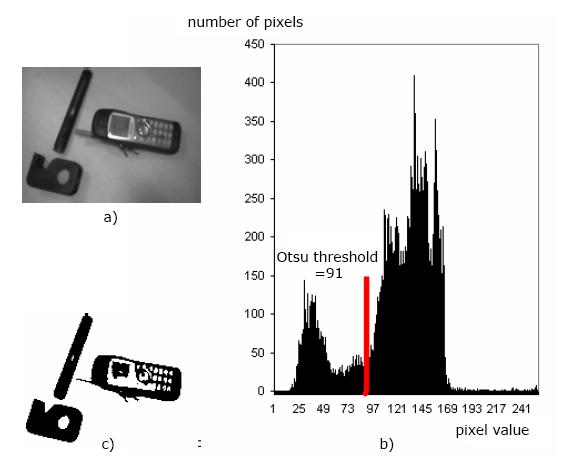
\includegraphics[width=100mm]{intel.jpg}
	\caption{Método de Otsu para definir o limiar}
Fonte: Intel~\cite{intel2017dev}
	\label{fig:otsu_ex}
\end{figure}

\subsection{Operações Morfológicas}
\label{sec:morfologicas}

Morfologia matemática é uma ferramenta para extrair componentes da imagem que são úteis para representação e descrição. É um método da análise de imagens que utiliza teoria dos conjuntos, podendo prover uma descrição quantitativa de estruturas geométricas. A maior parte das operações morfológicas são baseadas em operações de expansão e encolhimento, e são principalmente utilizadas em imagens binárias~\cite{owens1997morphology}.

Essas transformações envolvem interações entre uma imagem a ser processada, e um conjunto estruturante, chamado de elemento estruturante. Este elemento costuma ser um disco circular no plano, mas pode ter qualquer forma~\cite{owens1997morphology}.

Algumas operações são importantes para descrever as operações morfológicas, elas são: A translação, a reflexão e o complemento. 

A translação de B por x é denominada \(B_x\). Sejam A e B subconjuntos de um conjunto \(Z^2\), ela é definida por:

\begin{displaymath}
B_x = \{c : c = b + x, \mbox{for } b \in B\}. 
\end{displaymath}

A reflexão de B, denominada $\hat{B}$ é definida por:
\begin{displaymath}
\hat{B} = \{x : x = -b, \mbox{for } b \in B\}. 
\end{displaymath}

O complemento de a é denominado $Ac$ e a diferença entre os conjuntos A e B é denominado $A-B.$

As principais operações morfológicas são a erosão e a dilatação. Essas operações são fundamentais para o processamento morfológico. Grande parte das operações morfológicas são baseadas nessas duas operações~\cite{gonzalez1977digital}.

A dilatação de uma imagem A pelo elemento estruturante B é dada por:

\begin{displaymath}
A \oplus B = \{x : {\hat{B}}_x \cap A \neq \varnothing \}. 
\end{displaymath}

Na dilatação, o objetivo é dilatar as fronteiras de um objeto, ou seja, aumentar a espessura dos objetos em primeiro plano de uma imagem. A dilatação ocorre ao percorrer a imagem de entrada com o elemento estruturante, se ao menos um \emph{pixel} sob o elemento estruturante tiver seu valor sendo 1, na imagem original, todos os \emph{pixels} sob o elemento estruturante vão ser marcados como 1 na imagem de saída~\cite{opencv2014morph}. Na Figura~\ref{fig:dilation_ex} pode-se ver um exemplo da operação de dilatação em uma imagem.

\begin{figure}[H]
	\centering
	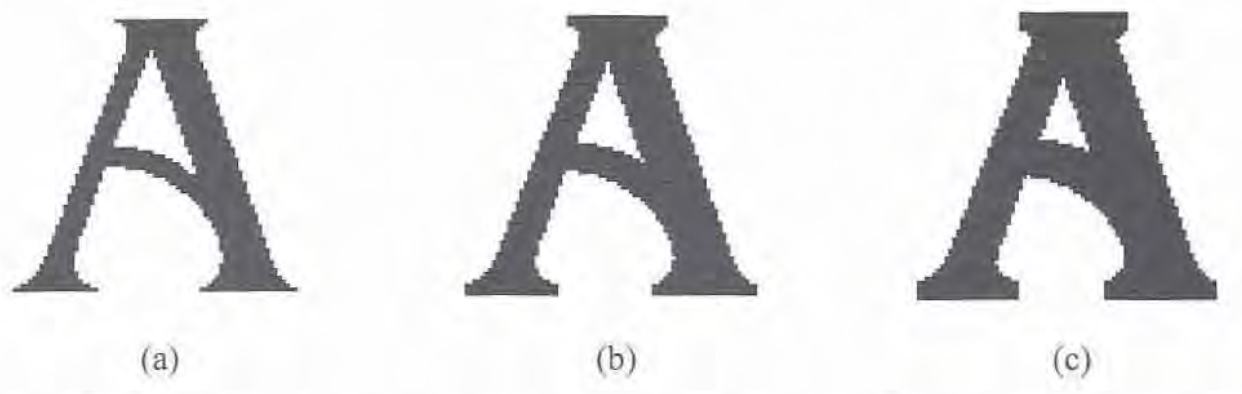
\includegraphics[width=100mm]{dilation.png}
	\caption{Dilatação em (b) com elemento estruturante de 3x3 e em (c) com elemento estruturante de 5x5}
Fonte: Efford~\cite{efford2000digital}
	\label{fig:dilation_ex}
\end{figure}

A erosão de uma imagem A pelo elemento estruturante B é dada por:
\begin{displaymath}
A \ominus B = \{ x : B_x \subseteq A \}. 
\end{displaymath}

A ideia por trás da erosão é, tal qual a erosão do solo, erodir as fronteiras de um objeto em primeiro plano. O elemento estruturante vai percorrer a imagem original e vai manter os \emph{pixels} da imagem de saída em 1 somente se todos os \emph{pixels} sob o elemento estruturante têm o valor de 1, caso contrário, essa parte da imagem é erodida, tem seus \emph{pixels} zerados. Dessa maneira os \emph{pixels} próximos das bordas vão ser descartados com base no tamanho do elemento estruturante e a espessura dos objetos em primeiro plano diminui~\cite{opencv2014morph}. Na Figura~\ref{fig:erosion_ex} pode-se ver um exemplo da operação de erosão em uma imagem.

\begin{figure}[H]
	\centering
	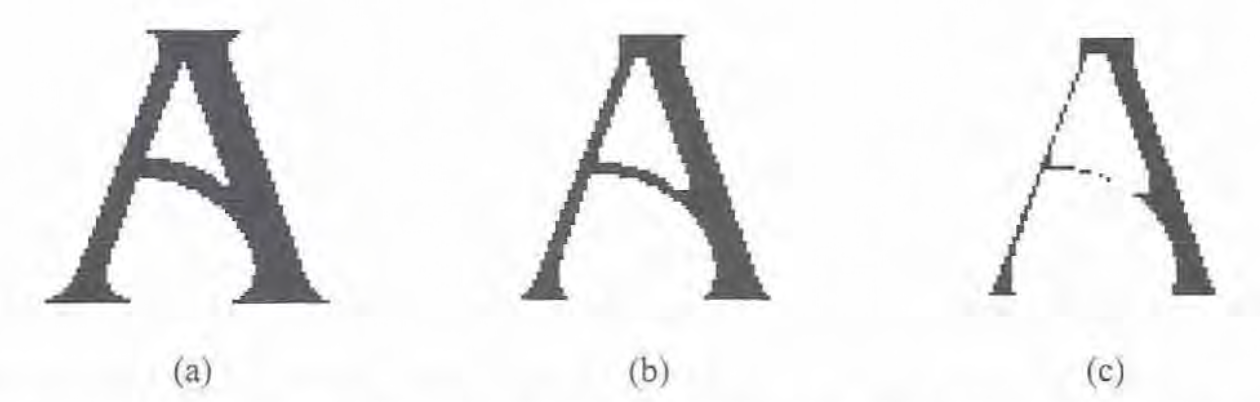
\includegraphics[width=100mm]{erosion.png}
	\caption{Erosão em (b) com elemento estruturante de 3x3 e em (c) com elemento estruturante de 5x5}
Fonte: Efford~\cite{efford2000digital}
	\label{fig:erosion_ex}
\end{figure}

Utilizando as operações de erosão e dilatação, é possível fazer as operações de abertura e fechamento. A abertura de uma imagem A, dado um elemento estruturante B, simbolizada por $A \circ B$, é feita pela erosão de A por B, seguida da dilatação de A por B, e pode ser representada pela equação:

\begin{displaymath}
A \circ B = (A \ominus B)\oplus B. 
\end{displaymath}

O fechamento de uma imagem A, dado um elemento estruturante B, simbolizada por $A \bullet B$, é feito pela dilatação de A por B, seguida da erosão de A por B, e pode ser representada pela equação:

\begin{displaymath}
A \bullet B = (A \oplus B)\ominus B. 
\end{displaymath}

Assim como a abertura, o fechamento também suaviza os contornos dos objetos, mas, ao contrário da abertura, ele geralmente funde  as protusões, eliminando pequenos buracos e preenchendo espaços no contorno~\cite{gonzalez1977digital}.

\section{Reconhecimento Ótico de Caracteres}
\label{sec:ocr}

Reconhecimento Ótico de Caracteres (\emph{Optical Character Recognition}, OCR)
resulta na conversão de textos em formato de imagem para o formato reconhecido por máquina. É o método mais eficiente para fazer o processamento de imagem para texto de acordo com Mohit et al.~\cite{mohit2015designing}.

Uma ferramenta conhecida de OCR é o
\emph{Tesseract}\footnote{https://github.com/tesseract-ocr/tesseract}. É um \emph{software} \emph{open source} de reconhecimento ótico de caracteres que suporta múltiplas línguas.  É essencialmente um algoritmo de comparação de \emph{templates}, e permite o auto treinamento de suas amostras de caracteres~\cite{ho2016intelligent}.

Neste trabalho, será implementado um \emph{software} de reconhecimento ótico de caracteres focado especificamente em reconhecer caracteres de placas de trânsito brasileiras utilizando aprendizado de máquina com o algoritmo \emph{K-Nearest Neighbors} que será fundamentado na Seção ~\ref{sec:knearest}

\subsection{K-Nearest Neighbors}
\label{sec:knearest}

\emph{K-Nearest Neighbors} é um dos algoritmos mais simples de classificação disponíveis para aprendizado supervisionado em aprendizado de máquina~\cite{opencv2014knearest}. Aprendizado supervisionado é tarefa de inferir uma função a partir de dados de treinamento rotulados. O algoritmo recebe um conjunto de exemplos como dados de treinamento e faz predições para os pontos não vistos com base nestes dados~\cite{mohri2012foundations}. A ideia do algoritmo \emph{K-Nearest Neighbors} é encontrar a combinação mais próxima de um determinado dado de teste em um espaço de dados~\cite{opencv2014knearest}.

Em um caso hipotético de aplicação do algoritmo existem duas classes: A classe dos quadrados azuis e a classe dos triângulos vermelhos. Este exemplo está ilustrado na Figura~\ref{fig:knearest_example}:

\begin{figure}[H]
	\centering
	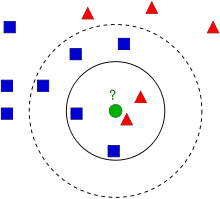
\includegraphics[width=50mm]{knn_theory.png}
	\caption{Exemplo de aplicação do K-Nearest Neighbors}
Fonte: Understanding k-Nearest Neighbour~\cite{opencv2014knearest}
	\label{fig:knearest_example}
\end{figure}

Pontos representando estas classes são espalhados em um espaço chamado de \emph{feature space}. Estes espaços são os espaços onde todos os dados estão projetados. Em um espaço de duas dimensões, como no exemplo, cada dado tem duas características, x e y. Em um espaço de três dimensões, cada dado teria 3 característica, em N dimensões, N características.

Na adição de um novo dado no \emph{feature space}, ele deve ser classificado como uma das duas classes. Este é o chamado de processo de classificação, no qual o algoritmo é aplicado.

Uma forma é o de verificar quem é o vizinho mais próximo. Na imagem, este seria o triangulo vermelho. Este método é chamado de \emph{Nearest Neighbor}, ou o vizinho mais próximo, pois a classificação só depende de um vizinho.

Outro método seria checar múltiplos vizinhos para ver quantos vizinhos de cada classe o novo dado possui. Na imagem, o triangulo vermelho é o vizinho mais próximo, mas, considerando múltiplos vizinhos, é possível classificar o novo dado na classe dos quadrados azuis, pois existem mais vizinhos desta classe. Este método é chamado de \emph{k Nearest Neighbors}, pois ele considera uma quantidade predeterminada \emph{k} de vizinhos para classificar seus novos dados~\cite{opencv2014knearest}.

Neste projeto o algoritmo \emph{K-Nearest Neighbors} é utilizado na implementação do reconhecedor ótico de caracteres encontrados em placas de transito brasileiras. São utilizados como dados de teste as letras maiúsculas e números na fonte \emph{Mandatory}, que é a fonte utilizada nas placas de carro brasileiras, e são aproximados os valores dos caracteres segmentados da placa com base nestes. Como haverá apenas um valor para cada classe, cada classe representando um caractere diferente, será utilizado apenas o vizinho mais próximo para classificar os caracteres. Tendo um conjunto de treinamento maior, é possível aumentar este valor.
 